% Listas Lineares


Listas Lineares
===============

\begin{definition}
\begin{tabbing}
Conjunto $\{\ell[0], \ell[1],...,\ell[n-1]\} :$\= $\forall k \in
\{0, 1,..., n-1\} \Rightarrow$\\
 \> o nó $\ell[k]$ é precedido por $\ell[k-1]$\\
\end{tabbing}
\end{definition}


Alocação sequencial: arranjo (vetor)
====================================

Um {\bf arranjo} armazena uma sequência de objetos, todos do mesmo
tipo, em posições consecutivas de memória.\\

``.C
#define N 5

int a[N];
``

\vspace{-.75cm}
\begin{center}
\small
$$a[0..n-1], 0\leq n\leq N$$
{\color<2>{gray}se $n=0$, arranjo {\bf vazio}}\\
{\color<1>{gray}se $n=N$, arranjo {\bf cheio}}\\
\end{center}

\begin{center}

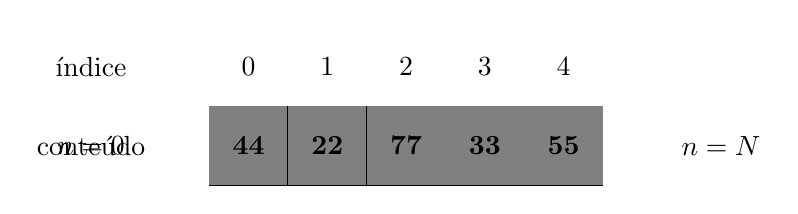
\begin{tikzpicture}
\def\shift{1cm}
\tikzset{every node/.style={minimum width=\shift, minimum
height=\shift}, ai/.style={draw}}
\foreach \i/\j in {0/44,1/22,2/77,3/33,4/55} {
 \node[ai] (a\i) at (\i*\shift,0) {};
 \node<2>[fill=gray]   at (\i*\shift,0) {\bf \j};
 \node [above of=a\i] (idx\i) {\i};
}

\node<1> [left of=a0,xshift=-\shift] {$n=0$};
\node<2> [right of=a4,xshift=\shift] {$n=N$};

\node<2> [left of=idx0,xshift=-\shift] {índice};
\node<2> [left of=a0,xshift=-\shift] {conteúdo};

\end{tikzpicture}

\end{center}

\end{frame}

Busca com sucesso
=================

\input{img/list-array-search-found}
  


Busca sem sucesso
================

\input{img/list-array-search-notfound}


Busca: Implementação em C
==========================

\lstinputlisting[frame=single,frameround=tttt,firstline=5,lastline=16,mathescape]{src/lista.c}


Análise: Busca sequencial em lista não ordenada
===============================================

\noindent O número de comparações de acordo com a posição na lista é

  $$C_N = {{1 + 2 + \ldots + N} \over N}, $$

\noindent  a partir da indentidade 

\note{from TAOCP1 pg 32}

 $$\sum_{0\leq j\leq n} (a + bj) = a(n + 1) + {1\over 2} bn (n + 1), $$

\noindent obtemos

  $$ C_N = {{N + 1} \over 2}.$$


Experimento: Busca sequencial em lista não ordenada
===================================================

fig from src/Cn.pdf
 
Alocação Encadeada: Lista Ligada
================================

\begin{block}{Modelo}

\bigskip
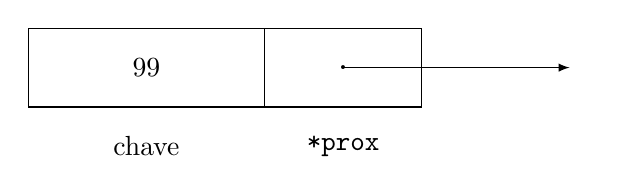
\begin{tikzpicture}
\tikzset{cel/.style={minimum width=2cm,minimum height=1cm,draw},
key/.style={cel,minimum width=3cm},
}

\node[key] (key0) {99};
\node[] [below of=key0] {chave};
\node[cel] (link0) [right of=key0,xshift=1.5cm] {{\LARGE .}};
\node[] [below of=link0] {{\tt *prox}};
\node (prox) [right of=link0,xshift=2cm] {};

\path[->,>=latex,draw] (link0.center) -- (prox);

\end{tikzpicture}

\end{block}

\bigskip
\begin{block}{Definição do Tipo de Dados}
\lstinputlisting[firstline=4,lastline=7,frame=single,frameround=tttt]{src/lista.h}
\end{block}


Lista Circula Ordenada: Inserção e Remoção: Ideia
==================================================
  animategraphics[step]{1}{img/list-linked-add-remove}{}{}     


Inserção em Lista Encadeada
===========================

\lstinputlisting[frame=single,frameround=tttt,firstline=29,lastline=38]{src/lista.c}

Análise: $\mathcal{O}(n)$.


Remoção em Lista Encadeada
==========================

\lstinputlisting[frame=single,frameround=tttt,firstline=40,lastline=48]{src/lista.c}

Análise: $\mathcal{O}(n)$.


Lista Encadeada: Busca: Ideia
===============================
  \input{img/list-linked-search-found}


Busca em Lista Ligada
=====================

\lstinputlisting[frame=single,frameround=tttt,firstline=17,lastline=28]{src/lista.c}

Análise: pior caso, $C_N = N$; melhor caso, $C_N = 1$.
